\documentclass{article}
\title{Fun Problem 1}
\usepackage{graphicx}



\begin{document}
\maketitle

We consider a regular tetrahedron $A$, that is, a polygon with four faces, all of which are equilateral triangles. Assume that the length of each edge of those triangles is $2r$. Now we consider four balls of radius $r$, each one of them centered at one of the four vertices of the tetrahedron. Note that each ball touches the other three.

 What is the volume of the solid that lies inside the tetrahedron but outside of all four balls?

\begin{figure}[h]
  \begin{center}
  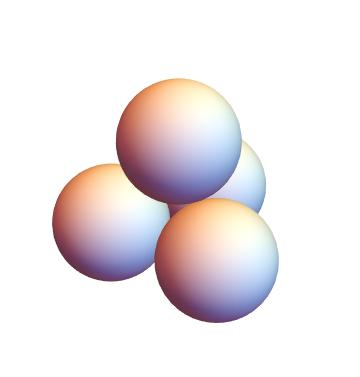
\includegraphics[scale=.5]{balls.jpeg}
  \caption{The four balls}
  \label{}
\end{center}

\end{figure}


\end{document}
